\documentclass{article}

\title{Initial Value Problems and Euler's Method}
\author{Jaden Krause}
\date{October 13, 2026}
\usepackage{float}
\usepackage{graphicx}
\usepackage{amsmath}
\makeatletter
\renewcommand{\topfraction}{0.95}       % Allow figures to use up to 95% of the page top
\renewcommand{\bottomfraction}{0.95}    % Allow figures to use up to 95% of the page bottom
\renewcommand{\floatpagefraction}{0.2}  % Allow a float page to be created even if it's only 20% full
\setcounter{topnumber}{4}               % Allow up to 4 figures at the top of a page
\setcounter{bottomnumber}{4}            % Allow up to 4 figures at the bottom of a page
\setcounter{totalnumber}{8}             % Allow up to 8 total figures per page
\makeatother
\begin{document}
\maketitle

\section{Introduction}
A common type of problem that is encountered in the study of differential equations is the Initial 
Value Problem (IVP). IVPs can also be one of the more simple types of differential equations to solve, as the 
initial condition (e.g. $y(0) = 1$) can be used to perform substituiton and isolate unknowns. However, many 
differential equations, and even some IVPs, are not as straightforward in solving. This is where Euler's Method comes into 
the discussion. 
\par
Euler's Method is used when no solution can be found to a differential equation by hand. It produces an approximation 
by computing the slope at a point of the function (using the derivative) and moving a step size $h$. It then calculates 
a new slope and moves again. Using this method, error increases as more approximations are performed, as the approximation 
moving along $h$ doesn't follow the true curve exactly. This tendency is shown in Figure 1, which demonstrates how the straight-line 
Euler's Method approximations deviate from a true function's line (in the figure, $e^{-x}$). The error of Euler's Method becomes much worse as 
the steepness of the curve rapidly changes.  A further discussion of the accuuracy of Euler's Method will be explored 
below. Euler's Method is defined as follows:
$$w_0 = y_0, \qquad w_{i+1} = w_i + hf(t_i,w_i)$$
Where $w_0$ and $y_0$ indicate the initial value, $w_i$ is the numerical approximation of the solution at the current time and
$w_{i+1}$ is the numerical approximation of the solution at the next time step $t_{i+1}$. $h$ is the step size, and $t_i$ 
is the time or independent variable at the $i$-th step. $f(t_i,w_i)$ is the differential equation function evaluated at the current 
time $t_i$ and current approximation $w_i$.
\begin{figure}[H]
    \centering
    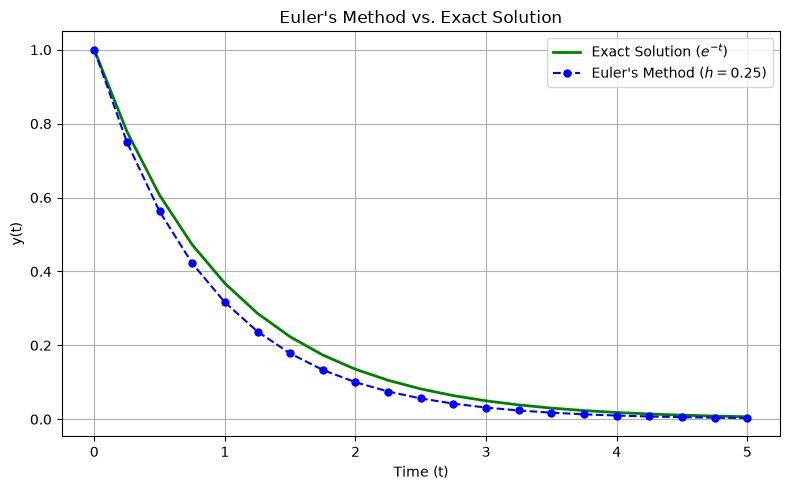
\includegraphics[width=0.75\textwidth]{EulerTendencies.png}
    \caption{Error Tendencies of Euler's Method}
\end{figure}

\section{The Problem}
The example problem used in this discussion is 
$$y' = ty + t^{3}, \qquad y(0) = 1$$
with initial condition specified above. Now, it is possible to find 
the solution to this equation by using differential equation solving skills. Thus, the exact solution is 
$$y(t) = 3e^{\frac{t^{2}}{2}} - t^{2} -2$$
We will be using this to compute the accuracy of Euler's method and compare how accuracy increases as $h$ decreases. 
Computing the error at several mesh resolutions ($h$ values), the values in Table 1 are obtained.
\begin{table}[htbp]
\centering
\caption{Convergence Performance of Euler's Method}
\begin{tabular}{|l|l|l|l|}
\hline
Step Size (h) & Euler Approx (t=2) & Exact Value (t=2) & Absolute Error \\
\hline
0.2 & 10.205253 & 16.167168 & 5.961915 \\
0.1 & 12.646560 & 16.167168 & 3.520609 \\
0.05 & 14.233190 & 16.167168 & 1.933978 \\
0.02 & 15.345157 & 16.167168 & 0.822012 \\
0.01 & 15.747429 & 16.167168 & 0.419740 \\
0.005 & 15.955047 & 16.167168 & 0.212121 \\
\hline
\end{tabular}
\end{table}
As demonstrated, smaller step sizes of $h$ result in improved accuracy. This is further seen in Figure 2, which shows how 
closely Euler's approximation gets to the true function at different values of $h$. 
\begin{figure}[H]
    \centering
    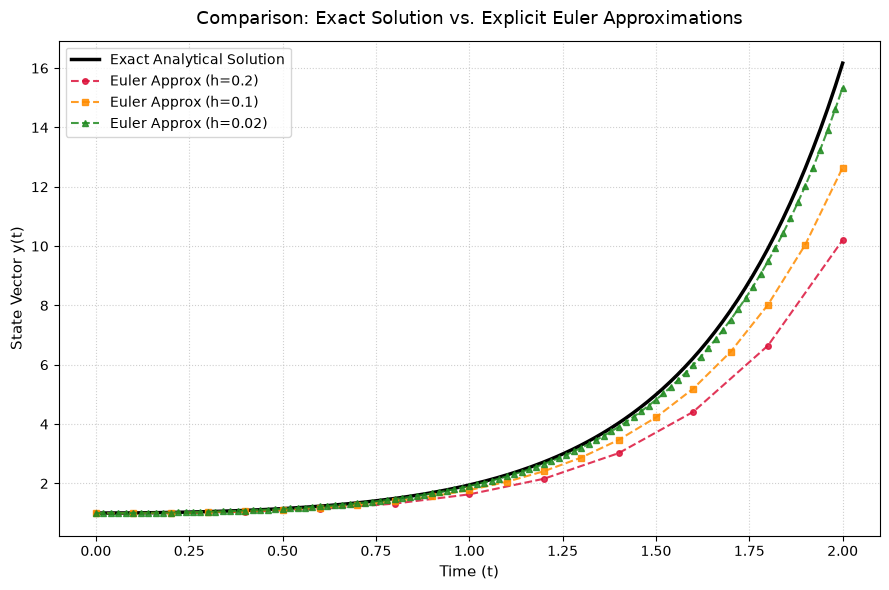
\includegraphics[width=0.75\textwidth]{EulervsExact.png}
    \caption{Euler's Method Compared to Exact Function}
\end{figure}

\section{Error Considerations}
Euler's Method is useful, but to use it effectively we must be familiar with the errors it is prone to and how to mitigate them. 
Locally, Euler's Method has a truncation error of order $\mathcal{O}(h^2)$. This is because, as $h$ decreases the approximation 
rapidly improves. Globally, however, Euler's Method is of order $\mathcal{O}(h)$. This results from the relationship between increasing 
accuracy as $\lim_{h \to 0}$, and decreasing accuracy as $n$ (number of steps) increases. This reflects the inverse relationship 
between $h$ and $n$, and is further exemplified by Figures 3 \& 4. Figure 5 shows the global, first-order convergence of Euler's 
Method and verifies the accuracy of our process of evaluation.
\begin{figure}[H]
    \centering
    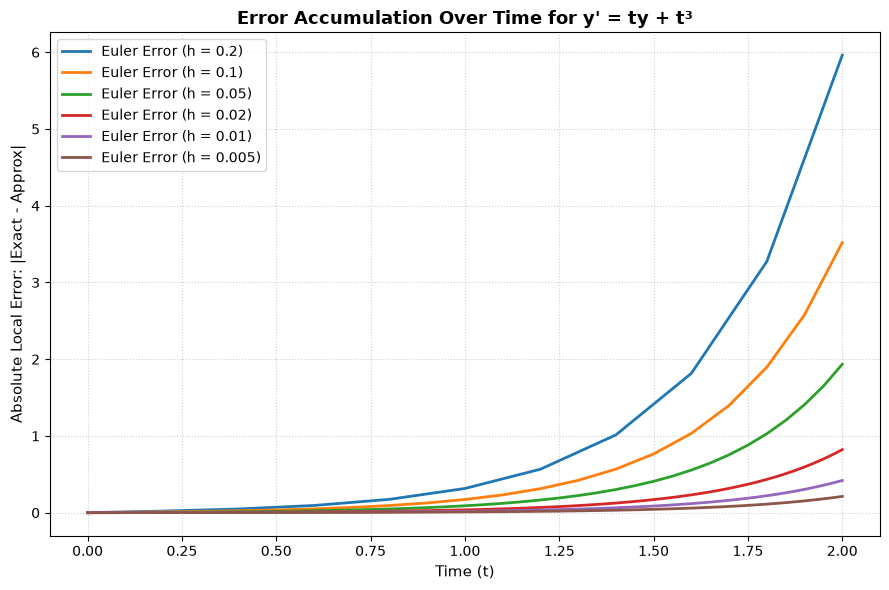
\includegraphics[width=0.75\textwidth]{ErrorvsTime.png}
    \caption{Error vs Time at different values of $h$}
\end{figure}
\begin{figure}[H]
    \centering
    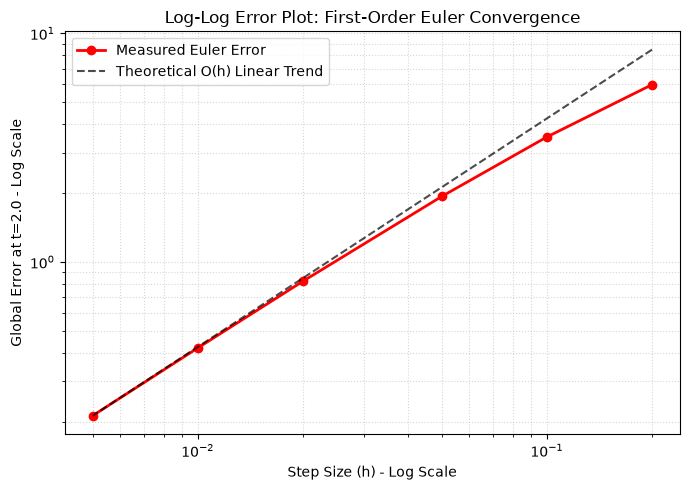
\includegraphics[width=0.75\textwidth]{ErrorvsH.png}
    \caption{Convergence of Euler's Method: Global First-Order}
\end{figure}

\begin{figure}[H]
    \centering
    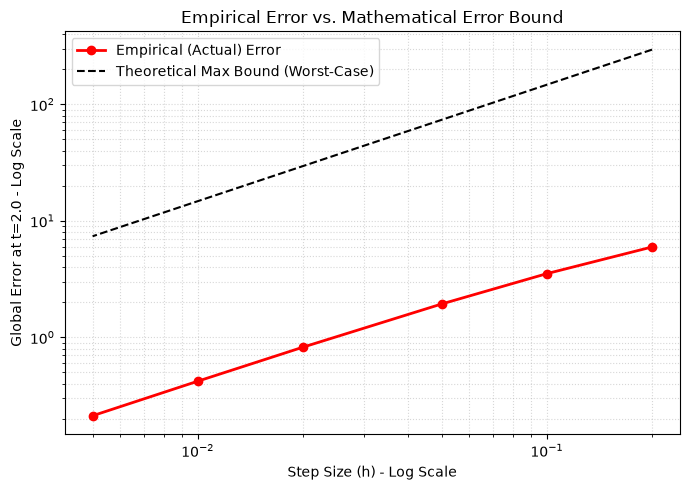
\includegraphics[width=0.75\textwidth]{EmpiricalvsTheoreticalError.png}
    \caption{Empirical Error Bound}
\end{figure}

\section{Conclusion}
In this paper, we analyzed the effectiveness of Euler's Method and applied it to an example problem. The relationship between 
error and $h$ was evaluated, and the local vs global convergence patterns of Euler's Method were considered. Euler's Method is 
overall, a consistent approximation method for functions, but it would still be desirable to find a method that follows the true 
curve better while not being overly complex to implement using computation.

\end{document}